%!TEX root = main.tex

\section{Especificación}
En esta sección veremos cómo funcionan las herramientas involucradas y cuáles son los puntos de extensión que proveen.

\subsection{Arquitectura de Mumuki}
Antes de empezar a hablar de la arquitectura, es necesario entender cómo se estructura el contenido dentro de la plataforma, ya que esto impacta en cada uno de los componentes.

El ejercicio es la mínima unidad de contenido: se trata de una descripción de un problema y una forma de evaluarlo. Desde el punto de vista del estudiante, consta de un título, una descripción del problema, una serie de ayudas adicionales y un corolario (que se muestra tras resolver el problema correctamente). Desde el punto de vista técnico, se estructura de la siguiente manera:

\begin{itemize}
  \caracteristica{Pruebas} evalúan que la solución resuelva el problema de forma correcta, es decir, que llegue al resultado esperado.

  Por ejemplo, si tenemos una función \codigo{dobleDe(numero)} que recibe un número y devuelve su doble, una prueba posible sería que \codigo{dobleDe(2)} da como resultado \codigo{4}.

  \caracteristica{Expectativas} evalúan que la solución resuelva el problema de forma adecuada, es decir, que se utilicen las herramientas correctas.

  Supongamos que ahora queremos hacer la función \codigo{cuadrupleDe(numero)}, que tome un número y devuelve su cuadruple, y queremos que el estudiante la implemente en términos de \codigo{dobleDe} (ya que multiplicar por 4 es lo mismo que multiplicar 2 veces por 2). En ese caso nuestro objetivo sería \codigo{cuadrupleDe(numero) \textit{debe usar} dobleDe(numero)}.

  \caracteristica{Código adicional} herramientas que el estudiante puede utilizar al escribir su solución. Pueden ser fruto de ejercicios anteriores o simplemente partes del problema que el docente quiera facilitar.

  Retomando el ejemplo anterior, la función \codigo{dobleDe(numero)} podría ser provista por el docente, ya que se supone que el estudiante pudo razonarla en el ejercicio anterior y sería tedioso que tuviera que volver a escribirla.
\end{itemize}

De los componentes mencionados en la introducción, sólo nos interesan el Atheneum y los \runner s ya que como vemos en la Figura \ref{fig:FlujoSubmission} son los que intervienen en el proceso que va desde el envío de la solución del estudiante hasta la obtención del resultado.

A grandes rasgos, la comunicación se realiza de la siguiente manera:
\begin{itemize}
  \item{El estudiante envia su solución, lo cual produce un POST HTTP hacia el Atheneum.}
  \item{El Atheneum envia otro POST HTTP al \runner\ correspondiente, agregando las pruebas, expectativas y código adicional del ejercicio.}
  \item{El \runner\ responde al pedido HTTP con el resultado de evaluar la solución, que puede ser: \codigo{errored} si el programa no compila, \codigo{passed\_with\_warnings} si el programa es correcto (pasa las pruebas) pero no utiliza las herramientas adecuadas o \codigo{passed} si es correcto y cumple con las expectativas.}
\end{itemize}

\begin{figure}
  \centering

  \begin{sequencediagram}
    \newthread{estudiante}{Estudiante}{}
    \newinst{atheneum}{Atheneum}{}
    \newinst{runner}{Runner}{}

    \begin{call}{estudiante}{Validar(solucion)}{atheneum}{resultado}
      \begin{call}{atheneum}{Validar(solucion, pruebas, expectativas, codigo\_adicional)}{runner}{resultado}
      \end{call}
    \end{call}
  \end{sequencediagram}

  \caption{Comunicación entre el estudiante, el Atheneum y un \runner.}
  \label{fig:FlujoSubmission}
\end{figure}

\subsection{Requisitos para poder implementar un \runner}
Para poder implementar un \runner, es necesario que el lenguaje cumpla ciertas características.

\sepfootnotecontent
  {GBB}
  {Acrónimo para GoBstones Board. Es un archivo de texto plano con un formato particular que permite especificar tableros.}

La primera de ellas: tiene que poderse ejecutar por línea de comandos, sin la intervención de un humano. Si bien esto puede sonar trivial cuando de lenguajes industriales se trata, no lo es para este tipo de herramientas didácticas. Suelen estar fuertemente acopladas con el entorno visual que proveen para programar, haciendo que no sea posible ejecutar fuera de allí (lo que imposibilita, por ejemplo, crear un \runner\ que ejecute un programa hecho en Scratch). Afortunadamente \pyGob\ sí cuenta con dicha posibilidad, pueden ejecutarse programas por la consola y visualizar el resultado en formato GBB\sepfootnote{GBB} o HTML.

Lo siguiente es poder probar que la solución del estudiante sea correcta. De un programa Gobstones pueden interesarnos validar dos cosas: dado un tablero inicial conocido, el problema tiene que llegar a un tablero final esperado (si se trata de un programa o un procedimiento) o tiene que retornar un valor esperado (si se trata de una función). Este tipo de pruebas se denominan unitarias y suelen ser escritas en algún framework específico del lenguaje con el que se está trabajando: JUnit para Java, rspec para Ruby, mocha para Javascript,etcétera. En este caso tuve que desarrollarlo yo, ya que hasta el momento no existía un framework así para Gobstones.

\sepfootnotecontent
  {AST}
  {Representación de árbol de la estructura sintáctica abstracta (simplificada) del código fuente, donde cada nodo del árbol denota una construcción que ocurre en el código fuente. La sintaxis es abstracta en el sentido que no representa cada detalle que aparezca en la sintaxis verdadera, omitiendo, por ejemplo, comentarios, espacios y saltos de línea.}

Por último, se tiene que poder analizar el código del estudiante para verificar si se cumplen las expectativas. La forma más sencilla de lograrlo es recorriendo el árbol de sintaxis abstracta (AST\sepfootnote{AST}), buscando que existan ciertos patrones. Si bien \pyGob\ ya proveía una manera de obtener el AST, tuve que solicitarle al equipo de desarrollo algunos cambios que comentaré más adelante.

\subsection{Cambios realizados en \pyGob}
\sepfootnotecontent
  {Abalorios}
  {En paralelo al desarrollo de este trabajo y sin saber de la existencia del mismo, surgió una iniciativa similar por parte del Lic. Pablo Barenbaum, docente de la cátedra Introducción a la Programación en UNQ. Al enterarnos de que estabamos trabajando en proyectos similares, se optó por pausar el desarrollo de Abalorios.}

\sepfootnotecontent
  {PullRequestHTML}
  {Pueden verse los cambios realizados en \url{https://github.com/gobstones/PyGobstones-Lang/pull/1}.}

La visualización HTML del tablero que proveía el intérprete era poco atractiva y distaba mucho de la identidad visual de Gobstones. Basado en la representación que el Lic. Pablo Barenbaum confeccionó para la herramienta Abalorios\sepfootnote{Abalorios}, creé una nueva representación (ver Figura \ref{fig:TableroHTML}) que luego fue integrada a la versión estable de \pyGob\sepfootnote{PullRequestHTML}.

\begin{figure}
  \centering
  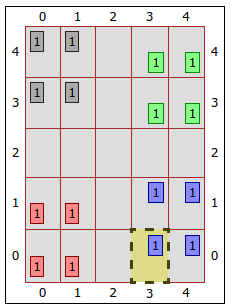
\includegraphics[scale=0.5]{images/tablero-html-viejo.png}
  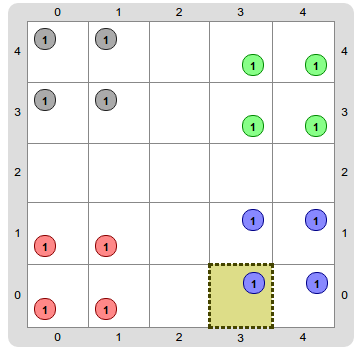
\includegraphics[scale=0.4]{images/tablero-html-nuevo.png}

  \caption{Representación HTML de un tablero Gobstones. A la izquierda, la versión implementada en \pyGob\ hasta la realización del presente trabajo; a la derecha, la nueva versión.}
  \label{fig:TableroHTML}
\end{figure}

\sepfootnotecontent
  {IssueAST}
  {Puede verse la discusión en \url{https://github.com/gobstones/PyGobstones/issues/32}.}

Con la generación del AST ocurrieron dos problemas puntuales, que fueron resueltos por el equipo desarrollador al poco tiempo de haberlos reportado\sepfootnote{IssueAST}.

El primero fue que además de generarse el AST se ejecutaba el código, inhabilitando la posibilidad de correr expectativas sobre programas sintácticamente válidos que arrojaban error en tiempo de ejecución. El siguiente problema fue que no era posible generar el AST de una única función o procedimiento, lo cual obligaba a tener que correr las expectativas sobre el código del estudiante y el provisto por el docente, sin poder diferenciar fácilmente qué parte se estaba analizando.
